\chapter{Lamello: Acoustic Sensing of 2D/3D Mechanisms}

\begin{quote}
A lamellophone (also lamellaphone or linguaphone, from the Latin root lingua meaning ``tongue", i.e., a long thin plate that is fixed only at one end) is any of a family of musical instruments.

The name comes from the Latin word ``lamella" for "plate" and the Greek root ``phonos" for ``sound". The name derives from the way the sound is produced: the instrument has a series of thin plates, or ``tongues", each of which is fixed at one end and has the other end free. When the musician depresses the free end of a plate with a finger or fingernail, and then allows the finger to slip off, the released plate vibrates.

--- ``Lamellophone" on Wikipedia
\end{quote}

\section{Preamble}
Moving towards more complex user interactions and sensing mechanisms, this chapter describes Lamello, which predicts the vibrational frequencies of 3D geometry and links those predictions to an acoustic sensing system. Lamello can be used to design interfaces with rich tangible feedback provided by mechanical input components that can be manipulated by users.

%We describe \emph{Lamello}, an approach for creating tangible input components that recognize user interaction via passive acoustic sensing. Lamello employs comb-like structures with varying-length tines at interaction points (e.g., along slider paths). Moving a component generates tine strikes; a real-time audio processing pipeline analyzes the resultant sounds and emits high-level interaction events. Our main contributions are in the co-design of the tine structures, information encoding schemes, and audio analysis. We demonstrate 3D printed Lamello-powered buttons, sliders, and dials. 

\section{Introduction}
%\valkyrie{How are mechanical interfaces important?  How are they seen today?}

Tangible input components like buttons and sliders
have advantages over ``flat'' interfaces like touch screens. They are critical for eyes-free interaction and muscle memory, and can improve task speed and precision \cite{klemmer-bodies}. Such devices typically comprise integrated assemblies of electronics, enclosures, and microcontroller code.

Recently, researchers have begun to explore acoustically sensing interactions---such as scratching---with digitally-fabricated objects that encode information in surface textures~\cite{harrison-acoustic,murray-smith-stane}. In this chapter, we extend this line of work from sensing surface features to sensing interactions with tangible components that users can push, slide, and turn.

Our technique, Lamello, integrates algorithmically-generated tine structures into movable components to create passive tangible inputs (Figure \ref{fig:lamello-pretty-components}). Manipulating these inputs creates sounds which can be captured using an inexpensive contact microphone and interpreted using real-time audio signal processing. Lamello predicts the fundamental frequency of each tine based on its geometry: thus, recognition does not require training examples. The decoded high-level events can then be forwarded to interactive applications. The name ``Lamello'' is derived from the Lamellophone family of instruments, which create sound through vibrating tongues of varying lengths. 

\begin{figure}[t]
  \centering
    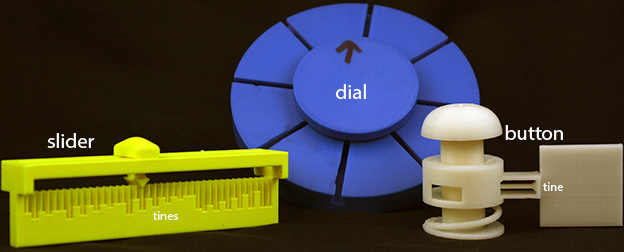
\includegraphics[width=\textwidth]{figures/lamello/fig1-labels-new.jpg}
   \caption{Passive tangible inputs that can be sensed acoustically. %\valkyrie{this one is shorter, which means more space for words! alt one is figures/newfig1.JPG}
   }
   \label{fig:lamello-pretty-components}
\end{figure}

Recognizing mechanically-generated sound for input has important limitations---only movement generates sound, so steady state cannot be sensed---but also appealing characteristics: Components can be fabricated from a single material (e.g., 3D printed ABS plastic), and ``wiring'' only requires attaching a microphone. In this chapter, we offer two important contributions:

\begin{enumerate}
\item a novel sensing mechanism driven by passive, plastic mechanisms that generate predictable sound when manipulated, and
\item design and fabrication guidelines for manufacturing compatible mechanisms, and a demonstration of several traditional input components sensed using our approach
\end{enumerate}

Our evaluation indicates that training-free recognition is possible, though our recognizer only has useful accuracy for a subset of tested tines.

    \subsection{The Geometry-Sensing Link}
    Lamello uses a predictive model which connects the geometry of a cantilevered beam (i.e., the ``tines'' used in this project) to a fundamental frequency when excited. We demonstrate the model, which assumes the beam is uniform, to be useful, in spite of the fact that tines fabricated on a 3D printer are not composed of uniform material. This pre-print modeling of frequencies allows training-free sensing of fabricated input devices using a microphone.
    
\section{Designing with Lamello}

\begin{figure*}[t]
  \centering
    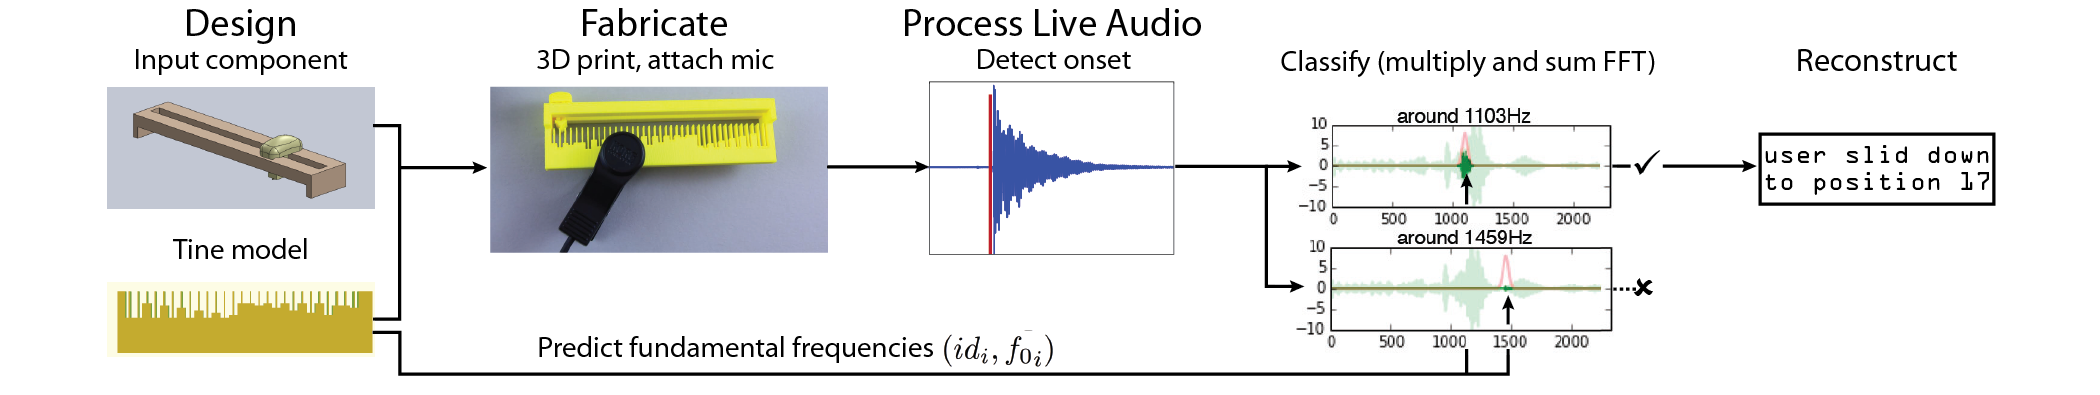
\includegraphics[width=\textwidth]{figures/lamello/systemdiagram-bh.png}
  \caption{Lamello reuses information between the design, fabrication, and audio processing steps to allow training-free passive acoustic sensing.}
  \label{fig:lamello-system}
  \vspace{-0.1in}
\end{figure*}

    \subsection{Users}
    
    Lamello targets makers, who are somewhat familiar with 3D modeling tools (e.g., SolidWorks or Google SketchUp for solid modeling, or openSCAD for programmatic design generation) and 3D printing. In its present, prototype form, Lamello also relies on users' familiarity with basic programming to create software interactions based on user input; it does not leverage record-and-replay as Midas does.
    
    Lamello can generate tine sets automatically; input component geometry---that is, everything that is \emph{not} a tine, like the track and header of a slider---can be derived from its library. The tines and additional geometry must right now be combined by hand. Power users with a more sophisticated understanding of solid modeling programs can generate their own tines by hand (and use Lamello's prediction tools to predict their final frequencies), or create new types of input component geometry to use with their tines.
    
    Once a designer fabricates an input device, the process of preparing it for sensing is simple: he simply places it near a microphone. Users do not need any experience with coding or audio. Lamello automatically predicts the frequencies of tines generated using our scripts, and provides a GUI interface to predict frequencies for hand-built tine geometries. The sensing software only needs the frequency and ordering information from the tines (again, this ordering information is automatically-derived if a user uses our scripts).
    
    To use the output of the sensing tool to control a program, users can either use a record-and-reply style of interaction (for example, using a graphical tool like OSCulator which requires no programming) or accept OSC messages in their own software for more nuanced control.
    
    \subsection{Design Walkthrough}
    
    %\valkyrie{the thing about lamello is that of course it doesn't have a cad tool in the same way. this will be interesting to write.} 
    We discuss the design possibilities of Lamello using a concrete running example: a designer wishes to test out a passive environmental input device for light controls. This input should be in the form of a slider, unpowered, and sensed using a sensor already present in the environment. He has a laptop in his living room to control other aspects of his connected home, so he will use its built-in mic as his sensor.
    
     \subsubsection{Customizing a Library Component}
    The designer opens openSCAD, a free and open source, well-documented CAD tool. He doesn't have much experience with openSCAD, but he opens one of Lamello's library component files: the slider. He needs to be able to input at least 15 different lighting positions, and he wants the slider a bit larger than it is by default, so he changes the values of a few variables in the model. 
    
     \subsubsection{Fabricating Tine-based Components}
    He sends his slider design to a 3D printer for fabrication. His printer is a model which can lay soluble support material, so he simply prints the full design, then performs the necessary post-processing to remove support material. Optionally, for users who don't have access to printers with soluble support, Lamello tines can be lasercut from Polyoxymethylene (Delrin) while only the user-facing mechanism is 3D printed. The two can be assembled afterwards with machine screws and nuts.
    
    \subsubsection{Connecting Hardware to Software}
    
    When his slider comes out of the printer, he sets it on the table next to his laptop and starts the Lamello sensing software, where he enters the material the tines are made of (3D Printed ABS Plastic) to complete the frequency predictions for his model's tines. As he slides the striker past tines, the sound is detected by the microphone in his laptop, which displays an illustration of the slider, with detected tine strikes highlighted.
    
    \begin{figure}
  \centering
    
\includegraphics[width=\textwidth]{figures/lamello/andrew-light.png}
  \caption{Our designer tests his lighting setup, holding the printed component in his hand with his laptop and microphone next to him, and observes as the lights change in brightness with each tine strike.} 
  \label{fig:lamello-andrew}
\end{figure}
    
    \subsubsection{Defining Interactions}
    
    To control his lighting system, our designer writes a quick script: he scales the output tine number of his Lamello comb to the input range of luminance for his lightbulb, and forwards those events on to the IP address of the light control bridge. After testing (see Figure \ref{fig:lamello-andrew}), he can affix the Lamello component to the wall nearby the laptop.
    
\section{Implementation}

    \subsection{The Lamello CAD tool}
    
    Lamello relies mainly on just two components: an openSCAD script which generates tine geometry, and a python script which predicts the fundamental frequency ($f_0$) of a tine based on its geometry. These tools can be executed together (the openSCAD script automatically calls the python script) or separately (in the case that a user creates his own tine geometry by hand in another program).
    
        \subsubsection{Tine Geometry Generation}
    
        Through the process of testing and refining our own designs for geometry, we extracted several high-level requirements for tines, described below. These requirements are enshrined in a simple geometry generation script, which we implemented in openSCAD. The script only requires that the user input the number of tines to be generated and the shape in which to generate them: the output is a 3D object which has that many tines of differing fundamental frequencies, which are arranged either linearly or radially. This is accomplished with 

        To generate sounds, we embed tine structures in input components (Figure \ref{fig:lamello-pretty-components}). Our tines are rectangular beams, attached at their base to the component and free to deflect at their top. Interacting with a component causes tine plucks; these vibrate the body of the component and are captured by a contact microphone.
        
        Tines can be arranged in configurations supporting different interactions (e.g., sliding, rotating, pressing).
        
        \subsubsection{Tine Frequency Prediction}

        We model a vibrating tine as an ideal cantilevered beam of uniform density in free vibration~\cite{meirovitch-analytical}: 

            \begin{center}
             $f_0 = \frac{1.875^2 \sqrt{\frac{E\frac{bh^3}{12}}{\rho (bh)L^4}}}{2\pi} \approx .1615 \sqrt{\frac{Eh^2}{\rho L^4}}$Hz
            \end{center}

            Fundamental frequency ($f_0$) is governed by several variables: tine height ($h$) and length ($L$), as well as material properties (density $\rho$, Young's Modulus $E$). Tine breadth ($b$) in fact does not affect final frequency. Our script's generated tine designs keep $b$ and $h$ constant, varying $L$ to achieve different frequencies. This makes the strength required to strike each tine roughly equal: if desired, a designer could make some tines thicker (and thus harder to strike) than others, offering another layer of physical feedback in an interface.

            Our prototypes are 3D printed, resulting in non-uniform material deposition. To test the applicability of our model, we compared predicted and observed $f_0$ for several tines printed on two uPrint SE Plus FDM printers using Stratasys ABSplus-P430 thermoplastic. We find an appropriate material parameter by minimizing the error between observations and measurements. Fitted $E$ values ranged from $9500$ to $15500$ based on print orientation and particular printer. The remaining error $\mu= 69.0Hz$ ($\sigma= 112.5Hz$) shows our model usefully applies to printed tines (see Figure \ref{fig:lamello-freqsgraph}). Estimation of $f_0$ can be further improved by measuring post-print with calipers.
            
            \begin{figure}[b]
 \centering
    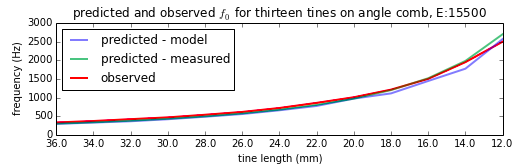
\includegraphics[width=3.25in]{figures/lamello/meirovitch-small.png}
 \caption{Three $f_0$s for tines in one print: predicted from model, predicted from post-print measurements, and observed. Error, model geometry: $\mu=$ 68Hz $\sigma=$ 36Hz, measured geometry: $\mu=$ 47Hz $\sigma=$ 45Hz.}
 \label{fig:lamello-freqsgraph}
\end{figure}

    This prediction of fundamental frequency can also be run separately on user-entered tine geometries.

        \subsubsection{Information encoding schemes}
        
        We use unique $f_0$s to differentiate buttons and directions on a D-pad. For position sensing, $f_0$ can increase across the range of motion (Figure \ref{fig:lamello-sliders} left). If more distinctions are needed than can be reliably recognized by varying $f_0$, we create de Bruijn patterns~\cite{debruijn-seqproof} (Figure \ref{fig:lamello-sliders} right). A de Bruijn sequence $D(k,n)$ is one which, given an alphabet size $k$ and a subsequence length $n$, contains each subsequence exactly once: we can uniquely infer sequence position from $n$ recognitions. This requires fewer $f_0$s, but more contiguous tine recognitions to determine user input.
        
        \begin{figure}
  \centering
    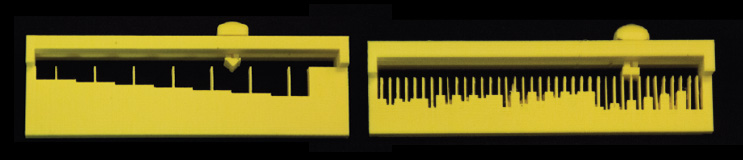
\includegraphics[width=3.25in]{figures/lamello/2sliders-sidebyside.jpg}
  \caption{We experimented with two different encoding mechanisms for sliders: linearly increasing sequences (left) and de Bruijn (right). de Bruijn sequences allow classification of fewer tine lengths, but require more consecutive tine recognitions to determine position and direction.}
  \label{fig:lamello-sliders}
\end{figure}

        \subsubsection{Integration of tines into larger components}

        We augmented several traditional input components: buttons, sliders, dials, and joysticks. Each has a ``striker" attached to the user-facing ``handle'' (Figure \ref{fig:lamello-allcomponents}). These strikers overlap with tine ends by $0.25-1mm$, balancing clear signal generation with easy interaction. Through testing, we determined that a triangular striker profile works best.

        The button has a rib around its shaft that strikes a tine when a user depresses it. The slider has a wiper that overlaps with the tops of tines (tines have different lengths, but are top-aligned). The dial works similarly, arranged radially rather than linearly. The D-pad derives from the button: a striker strikes a tine on the base as the user moves the handle up, down, left, or right.
        
        \begin{figure}
  \centering
    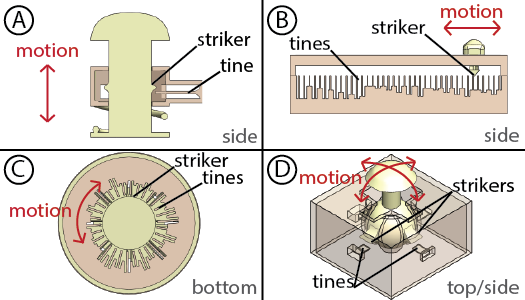
\includegraphics[width=\columnwidth]{figures/lamello/component-schematics.png}
  \caption{The Lamello technique can be used to sense a variety of physical motions, including up/down on a button, back/forward on a slider, and rotation on a dial or scroll wheel. Four tines used together can sense up, down, left, and right on a direction pad. %\valkyrie{we could cut parts of this figure, given that we never use buttons or joysticks for experiments. thoughts?}
  }
  \label{fig:lamello-allcomponents}
\end{figure}

        All components we created are parametrically-described models that can be modified to have, for example, more tines on a dial, a longer slider body, or a more robust button spring. Thus, our components can be customized, even without significant experience using 3D modeling software.

    \subsection{The Lamello Hardware}
    
    On the hardware side, Lamello requires both the fabricated input components and the sensing mechanism (i.e., the microphone).
    
    \subsubsection{Lamello's Sensing Apparatus}
    
    Lamello is designed to take advantage of sensors that already exist in an environment, specifically microphones. No custom hardware is necessary to sense Lamello-based inputs. Our initial tests leveraged cheap contact mics used for musical instruments clipped to the components, while we have since performed informal tests with thru-air microphones present in laptop computers. Audio sensing additionally presents more of a challenge, as it necessitates time- and frequency-domain analysis on a device with non-negligible computational ability, unlike the simple thresholded on/off of Midas. We describe our algorithms below.

    The audio signal of a tine strike is characterized by an initial transient---a short high energy sound across a wide range of frequencies---followed by free vibration with a local long-decay energy peak at the tine's resonant frequency (Figure \ref{fig:lamello-transient}). Conceptually, our recognizer detects a transient, finds the dominant resonant frequency after the transient passes, and compares it to predicted tine frequencies.
    
    
\begin{figure}
  \centering
    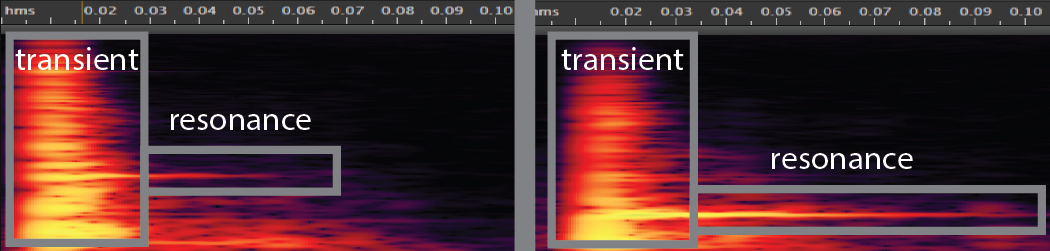
\includegraphics[width=\textwidth]{figures/lamello/transient-resonance.png}
  \caption{Two typical tine strikes (100ms): high-frequency (left) and low-frequency (right). We mark transients and resonance. Note the higher frequency has less energy (darker colors) and faster decay (shorter).} 
  \label{fig:lamello-transient}
\end{figure}

    Our audio processing pipeline, written in Python, uses basic frequency-domain features for classification. We sample our contact microphone at $16000Hz$. Our frames (sets of samples captured for analysis) are 2048 samples ($128ms$), and our hop length (offset between successive, overlapping frames) is 800 samples ($50ms$), for a frame overlap of $61$\%. Analyzing a frame takes $5ms$, plus additional latency incurred by sound hardware. In addition to the real-time audio stream, our recognition algorithm also takes an ordered list of $(id_i,{f_0}_i)$ tuples describing the tine ordering and fundamental frequencies of a component as input.

    For each frame, we first determine if a tine strike is present using a standard onset detector (with an empirically-determined amplitude threshold). Once an onset is detected, we wait 2 frame hops for the transient response to pass.
    
    We classify the subsequent frame (computation time: $5ms$). Our best-case onset-to-classification latency is therefore $2 * 50ms + 5ms = 105ms$. In practice, we have seen latency of $107.3ms$ ($\sigma$=$9.67ms$). Our sound card and the \emph{PySoundCard} driver introduce latency as they collect and report blocks: one could reduce overhead with optimized sound drivers and sample block sizes.

    To classify, we compute a Fast Fourier Transform on the window, then normalize the FFT bin values, such that they represent fractions of overall audio energy. For each possible tine $id_i$, we generate a new measure: the dot product of the scaled FFT and a Gaussian centered at the bin for ${f_0}_i$, which represents the fraction of audio energy $e_i$ in the neighborhood of ${f_0}_i$. To account for lower energy at higher frequencies, we use a scaling factor proportional to the frequency and a $\sigma$ for the Gaussians empirically determined per component, giving an adjusted list of ${e_i}_{adj}$. 

    Mapping a recognized tine identity $id_R=argmax({e_i}_{adj})$ to user actions is straightforward. For buttons and joysticks, $id_R$ maps directly to a discrete input (press, up, down, left, or right). Similarly, for dials and sliders that encode position with linearly increasing tine lengths, $id_R$ maps to a unique position. For dials and sliders that use a de Bruijn sequence $D(k, n)$, we use each sequence of $n$ recognized tines to determine the corresponding position within the sequence (i.e., recognized tines are remembered in order, and this order is compared to the known order of tines on the slider to determine a user's position). For buttons and joysticks, $id_R=argmax(p_R)$ maps these tine probabilities directly to a discrete input event (press, up, down, left, or right), while for sliders and dials the recognized tine, history, and layout are considered in order to generate a progress event ($14\%$, $58\%$, etc.).
    
    \subsubsection{Sensing Accuracy}
    
    To determine whether Lamello tines can be classified reliably, we performed an accuracy test using Lamello controls.

\begin{table}[b] 
  \begin{center}
  \small
  \begin{tabular}{ l || c | c || c | c }
  
Control & $P_{4tines}$ & $R_{4tines}$ & $P_{7tines}$ & $R_{7tines}$\\
\hline
FDM Slider & 93\% & 90\% & 49\% & 56\% \\  
FDM Dial & 90\% & 85\% & 63\% & 54\% \\  
Plucked Delrin & 98\% & 97\% & 72\% & 73\% \\
  \end{tabular}
  \end{center}
  \caption{Recognition precision and recall of our printed input components using model geometry-predicted frequencies.}
  \label{fig:lamello-recognition}
  \vspace{-0.1in}
\end{table}

We recorded 10 strikes for each tine on a printed dial and slider, and a laser-cut Delrin slider. Printed components were actuated with their strikers; Delrin tines were hand-plucked to determine effects of different striking methods. We classified each strike and report classification accuracy in Table~\ref{fig:lamello-recognition}.

We achieve promising accuracy (precision = 93\%, recall = 90\%) with a four-tine slider (predicted frequencies $924$, $1103$, $1340$, and $1662Hz$). This suggests that useful interaction with Lamello is within reach. However, precision and recall rates are much lower on a set of 7 tines with frequencies above $2kHz$: %including frequencies $2116$, $2784$, and $3827Hz$. 
the recognizer fails to classify higher $f_0$, which have lower energies and shorter decays (Figure ~\ref{fig:lamello-recall_rates}).

\begin{figure}[t]
  \centering
    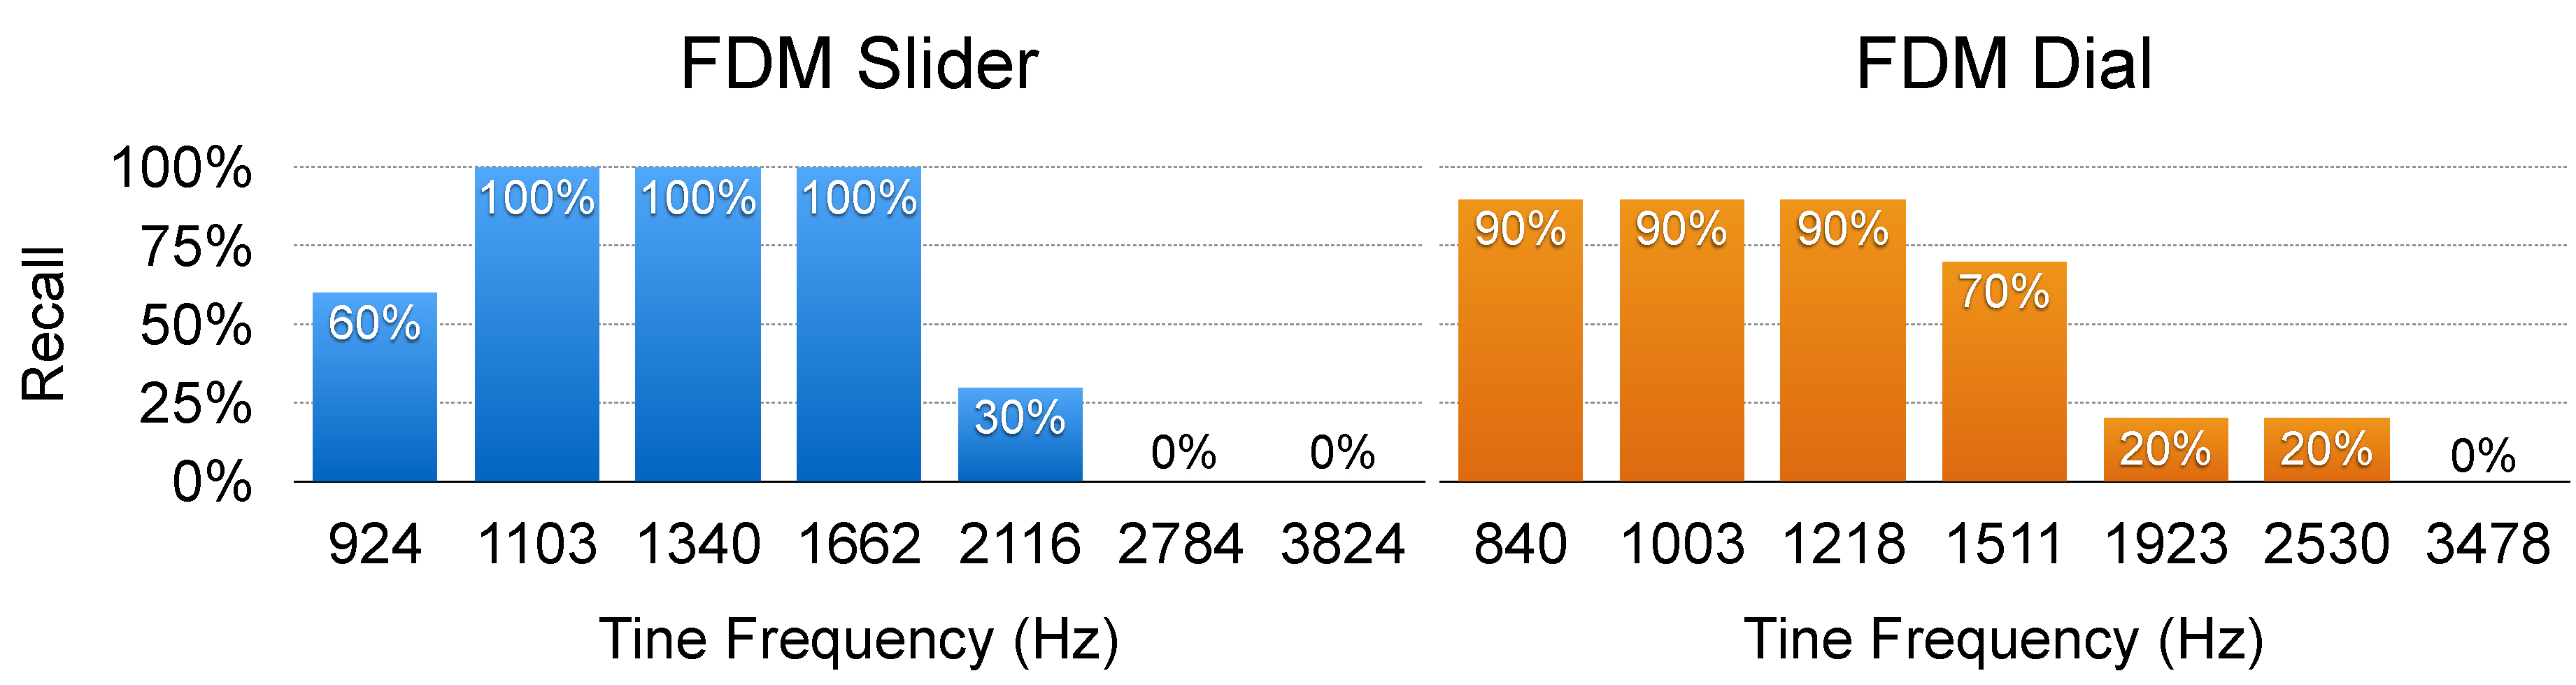
\includegraphics[width=4in]{figures/lamello/fig6.pdf}
  \caption{Per-tine recall for striking Lamello slider and dial tines. We observe high recall for low-frequency subsets of tines.}
  \label{fig:lamello-recall_rates}
\end{figure}

    We also noted that our hand-plucked Delrin tines outperformed tines hit with our striker designs: this suggests that our striker mechanism could use improvement. An additional way of improving these accuracy figures would be to model the way sound travels through \emph{the object itself}. Because we are using contact microphones, we are collecting sound waves travelling through the material rather than through the air. While this reduces sensitivity to outside noise, its accuracy can be affected by the particular designs of the components. In practice, all our different component designs had similar accuracy, which may indicate that for objects on the scale of input components designers need not worry about the particular acoustics of their design. However, for integrating Lamello-style components into larger input devices this may become a concern.

    \subsubsection{Fabricating Lamello-compatible Components}
    
    As mentioned, most of our prototype Lamello tines are 3D printed in FFF-extruded ABS plastic. While our $f_0$ predictive model works sufficiently well in spite of the non-uniformity of the material, tines printed in some orientations may break (see Figure \ref{fig:lamello-break}), and may need special calibration as their Young's Modulus ($E$) is likely to differ.
    
    \begin{figure}
  \centering
    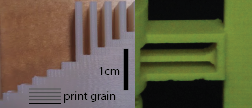
\includegraphics[width=3in]{figures/lamello/fab.png}
  \caption{Tines printed in some orientations may be prone to breaking: in particular, inter-layer adhesion is weaker than within-layer adhesion for 3D printing (left). Breakage can be mitigated by filleting tine corners instead of having them meet the body at right angles (right), but this can require additional details in the frequency prediction model.} 
  \label{fig:lamello-break}
\end{figure}
    
    Other printing or fabrication processes may not be orientation dependent. We have laser cut tines from Polyoxymethylene (Delrin) sheets, integrating these tine strips into 3D printed components using machine screws as fasteners. Tine sizes are similar between ABS-printed and lasercut objects, as laser cutting caused heat deflection in smaller feature sizes. Smaller tine sizes and higher frequencies may be achievable using different fabrication processes, e.g., injection molding or MEMS micromachining. We leave these investigations to future work.

\section{Evaluation}

    \subsection{Cost-Effective}
    Lamello-based components do not require dedicated sensing hardware: they can be sensed using microphones already present in laptops or, with additional software engineering, in smartphones. Each physical microphone can also be shared among multiple components, as a it need not be physically attached to a single input to acoustically sense it.
    
    The components themselves are also inexpensive, as ABS plastic for 3D printing costs approximately \$$50/kg$, and each of our example inputs weighs roughly an ounce. The polyoxymethylene sheets we experimented with for our laser cutter are approximately \$$10/ft^2$.
    
    \subsection{Fast}
    Input components built using this technique do not require post-processing. The time from design to functioning input is limited mainly by the speed of the 3D printer (while each of our sliders required only 2 hours to print, the joystick took 8). Once the print is completed and the support material removed, the technique does not require training---it relies on $f_0$s predicted from geometry rather than empirically determined---, and the components can be used right away. In the case that designers elect to create their components by assembling lasercut tines with 3D printed mechanisms, the assembly requires simply snapping the tines in (in the case of the dial, see Figure \ref{fig:lamello-laser}, left) or attaching a few screws (for the slider, see Figure \ref{fig:lamello-laser}, right).
    
\begin{figure}
  \centering
    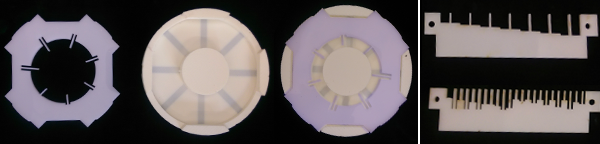
\includegraphics[width=\textwidth]{figures/lamello/lamello-laser.png}
  \caption{Lasercut tines can be integrated with 3D printed bodies. Left, lasercut dial tines can snap into a 3D printed body (lasercut tines are white, blue color added for clarity). Right, lasercut slider tines can be attached with clips or screws through their mounting holes.} 
  \label{fig:lamello-laser}
\end{figure}
    
    In future work, we hope to improve and deploy the Lamello CAD tool to gain insights about its legibility for users.

    \subsection{Flexible}
    We successfully used Lamello to create a variety of input components: buttons, sliders, dials, and joysticks. By combining and modifying their primitive actions (pushing, sliding, turning, and rocking), a designer could employ Lamello to sense components like scroll wheels or direction pads.
    
    To explore the utility of our technique, we used a Lamello slider and mouse emulation to control a Pong game. The achieved latency was sufficient for simple gameplay; however, Lamello may be better suited to provide input for applications such as volume or lighting control (as described in Design Walkthrough, above), where some latency and occasional misclassified events are acceptable.

\section{Discussion}

Initial experiments with Lamello are encouraging: components augmented with tines are easy to print and use, and tines produce unique, predictable frequencies. However, classification accuracy still needs improvement, and may require a new approach for $f_0>2kHz$.

    \subsection{Sweet Spots}

    Lamello opens opportunities to design tangible, mechanical interfaces cheaply and quickly, without the need to train a machine learning model for sensing. This technique is uniquely suited to creating simple, unpowered inputs in environments where microphones, such as those in laptops or, with additional engineering, cell phones, are already present. This includes applications in the Internet of Things or Smart Home, as we described in the scenario above in \emph{Designing with Lamello}. These inputs can be made more durable or more cheap as required by the application: the same 3D models can be fabricated in a variety of materials as desired.
    
    Like Midas's inputs, Lamello designs can be sized appropriately for the situation: they are not pre-fabricated like sensors for Arduino \cite{arduino} or those used in d.tools \cite{hartmann-dtools}, but rather can be stretched or shrunk or otherwise customized to fit perfectly with a larger design or requirement.
    
    Fabrication of these devices is fast, and they don't require training.
    
    \subsection{Limitations}
    
     We have identified several sources of errors to address in future work:

    \subsubsection{Striker mechanism could be more robust}
    In our experiements, finger-plucked tines had a higher rate of recognition than striker-actuated ones. This suggests that striker-created noise contributes to misclassifications, and future work may explore alternative geometries that create less friction noise.

    \subsubsection{Audio signal attenuates as it travels through component body}
    While microphones placed at opposite ends of a printed slider produce similar overall accuracy, tines are more correctly classified by the closer microphone. Though we could not directly correlate microphone distance and signal RMS energy, this fact suggests that minimizing the distance between a microphone and the tines to be sensed may improve accuracy.

    \subsubsection{Resonance and harmonics interfere with classification}
    Struck tines exhibit an energy peak at the predicted $f_0$, but their frequency spectrum is considerably more complex due to harmonics, component resonance, and other unmodeled material effects (e.g., the layered construction of 3D prints). Competing with non-fundamental vibrations is most problematic for short tines, whose resonant frequencies have lower energy. Future work can also probe optimal frequency distributions to avoid overlap between tine harmonics.

    \subsubsection{Unable to sense static configuration, continuous changes, or directionality}

    The Lamello approach can only detect position \emph{changes}---it cannot sense static configurations as they do not create sound. Continuous inputs are also unfeasible with the tine-based design: individual tines must be struck to localize a user's movement.
    
    We currently also cannot distinguish between the two directions in which a tine can be struck. We believe this could be remedied with ``sided'' tine geometry (i.e., asymmetric tine profiles), however this change would require a more sophisticated predictive model and additional inquiries into suitability for 3D printing.
    
    \subsubsection{Does not support multiple inputs simultaneously}
    Use of thru-air microphones based in laptop, tablets, or smartphones in the place of contact microphones could open applications beyond prototyping (e.g., custom controllers for tablet games). However, filtering out environmental noise collected by thru-air microphones is a challenge, and de-interlacing multiple simultaenous input components (e.g., if a button and slider are activated at the same time) will require more sophisticated signal processing than we have described here.
